\RequirePackage{luatex85}
\documentclass[tikz]{standalone}
% Default preamble
\usepackage{pgfplots}
\pgfplotsset{compat=newest}
\usepgfplotslibrary{groupplots}
\usepgfplotslibrary{polar}
\usepgfplotslibrary{smithchart}
\usepgfplotslibrary{statistics}
\usepgfplotslibrary{dateplot}
\usepgfplotslibrary{ternary}
\usepackage[T1]{fontenc}
\usepackage{lmodern}
\begin{document}
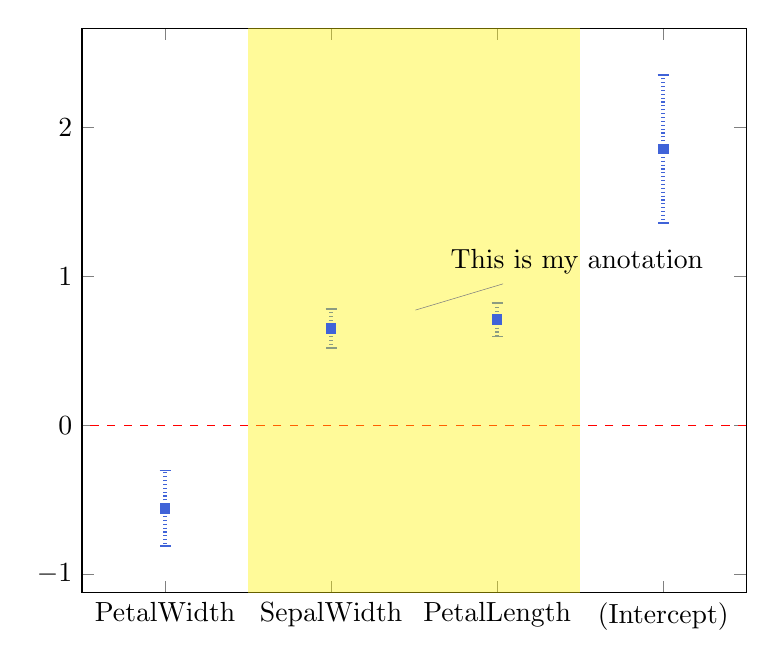
\begin{tikzpicture}
\begin{axis}[title style={}, xlabel style={}, ylabel style={}, xticklabel style={}, yticklabel style={}, width={240pt}, height={204pt}, symbolic x coords={PetalWidth,SepalWidth,PetalLength,{(}Intercept{)}}, xtick={PetalWidth,SepalWidth,PetalLength,{(}Intercept{)}}, xmin={{[normalized]-0.5}}, xmax={{[normalized]3.5}}, scale only axis]
    \addplot[only marks, mark={square*}, mark options={mark size={1.75pt}, line width={0pt}, fill={rgb,255: red, 64; green, 99; blue, 216}, fill opacity={1}, draw={rgb,255: red, 64; green, 99; blue, 216}, draw opacity={1}}, error bars/error mark={|}, error bars/error mark options={mark size={2.0pt}, solid, line width={0.6pt}, fill={rgb,255: red, 64; green, 99; blue, 216}, fill opacity={1}, draw={rgb,255: red, 64; green, 99; blue, 216}, draw opacity={1}}, error bars/error bar style={draw={rgb,255: red, 64; green, 99; blue, 216}, draw opacity={1}, densely dotted, line width={1.5pt}}, draw={rgb,255: red, 64; green, 99; blue, 216}, draw opacity={1}, line width={0.5pt}, error bars/y dir={both}, error bars/y explicit]
        coordinates {
            (PetalWidth,-0.5564826601670136) +- (0,0.25207883587827457)
            (SepalWidth,0.65083715931332) +- (0,0.13171828828576693)
            (PetalLength,0.7091319591367369) +- (0,0.11209691841092581)
            ({(}Intercept{)},1.8559974929171883) +- (0,0.49562225706654334)
        }
        ;
    \draw[dashed, red] ({rel axis cs:1,0}|-{axis cs:{[normalized]0},0}) -- ({rel axis cs:0,0}|-{axis cs:{[normalized]0},0});
    \draw[draw={none}, fill={yellow}, opacity={0.4}] ({rel axis cs:0.25,0}|-{rel axis cs:0,1}) rectangle ({rel axis cs:0.75,0}|-{rel axis cs:0,0});
    \draw node[pin=45:{This is my anotation}, inner sep=0, outer sep=0] at ({rel axis cs:0.5, 0.5}) {};\end{axis}
\end{tikzpicture}
\end{document}
